\chapter[Chemostat]{The chemostat\\[0.5cm] Some notions of phase plane analysis}
\label{chap:chemostat}



\section{The chemostat}

A chemostat consists in one main chamber (called a vessel), in which some microorganisms (bacteria, plankton), typically unicellular, are put, together with liquid and nutrient.
The contents are stirred, so nutrient and organisms are well-mixed.
Organisms consume the nutrient in their environment, which causes them to grow and multiply.
\begin{figure}[htbp]
\begin{center}
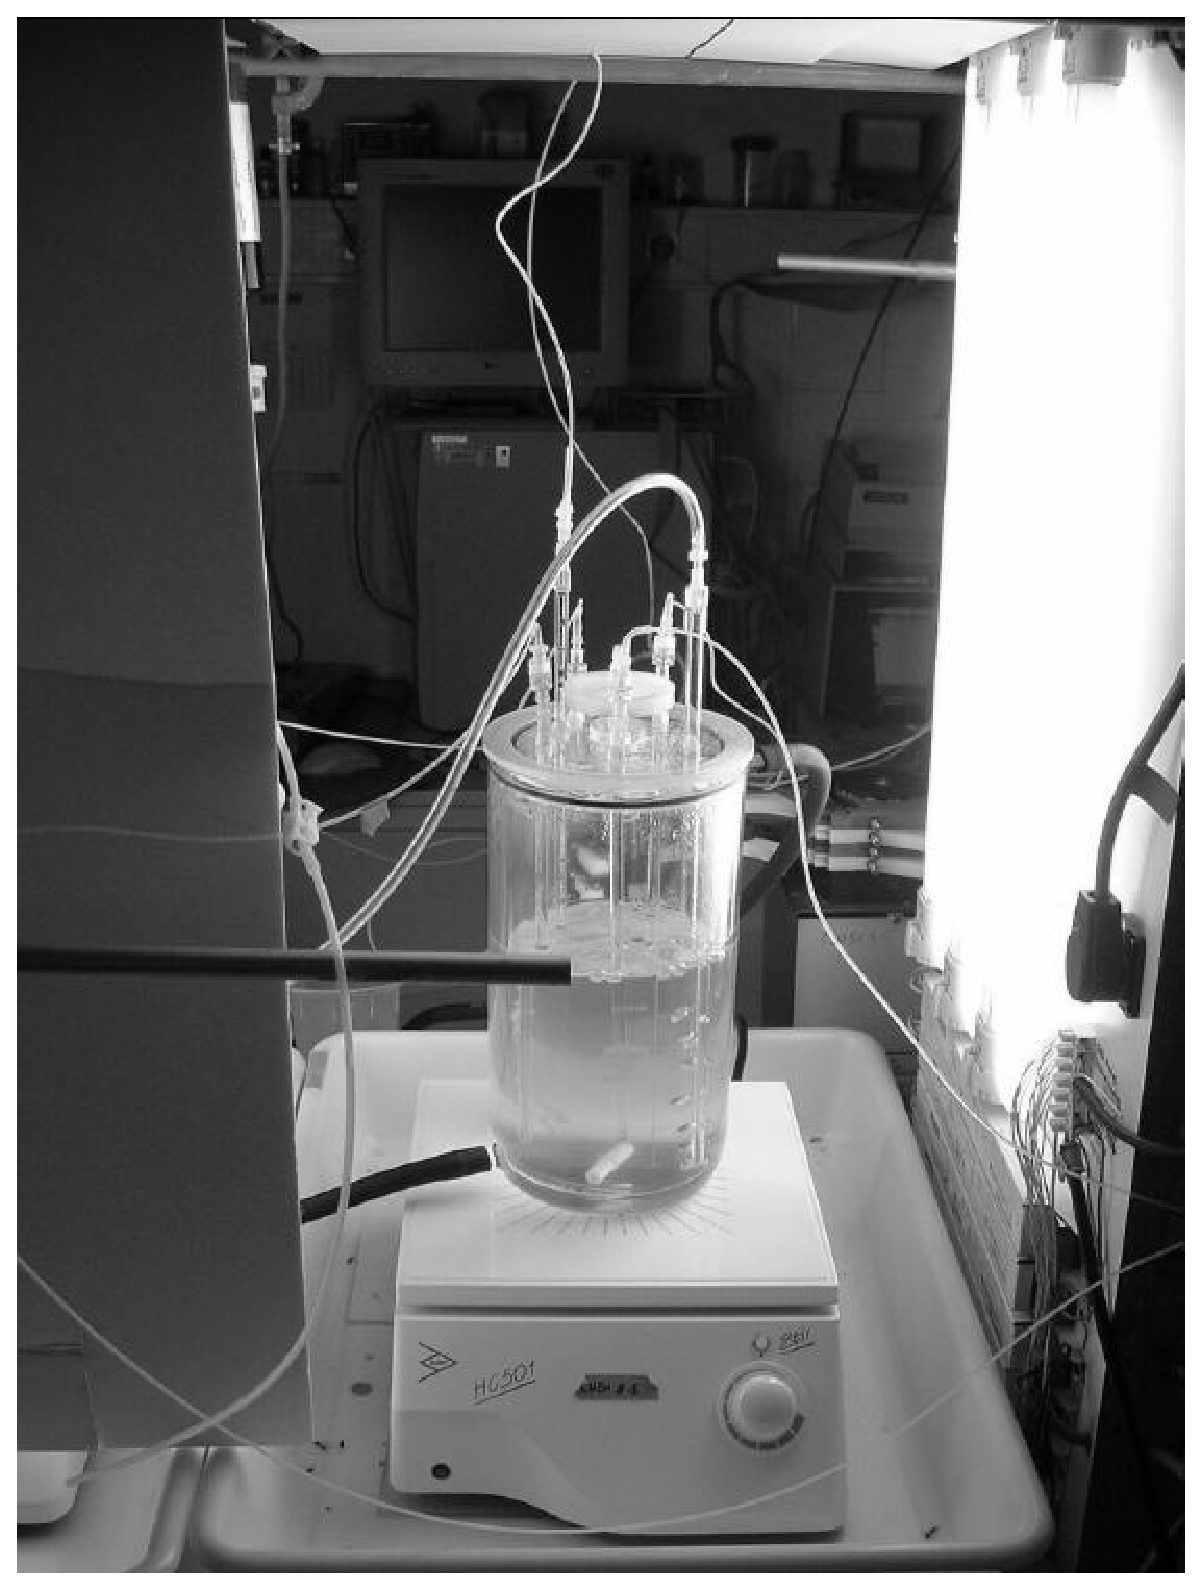
\includegraphics[height=0.45\textheight]
{../figs_05_chemostat/chemostat}
\caption{A chemostat operating at the Laboratoire
Oc\'eanographique de Villefranche sur Mer, France.}
\end{center}
\end{figure}
Two major modes of operation:
\begin{itemize}
\item \emph{Batch} mode: let the whole thing sit.
\item \emph{Continuous flow} mode: there is an input of fresh water and nutrient, and an outflow the comprises water, nutrient and organisms, to keep the volume constant.
\end{itemize}
Chemostats are very popular tools.
\begin{itemize}
\item Study of the growth of micro-organisms as a function of nutrient, in a very controlled setting.
\item Very good reproducibility of experiments.
\item Used in all sorts of settings. Fundamental science, but also, for production of products.
\end{itemize}


\section{Batch mode}
\subsection{Model with no cell mortality}
We make the following assumptions. Organisms, whose concentration is denoted $x$, are in the main vessel. Limiting substrate has a concentration in the vessel denoted $S$. There is homogeneous mixing of the contents of the vessel, so that nutrient is readily available to all organisms at the same  concentration. Therefore, spatial aspects can be neglected. Organisms uptake nutrient at the rate $\mu(S)$, a function of the concentration of nutrient around them.
First, we assume no death of organisms. The model then is
\begin{subequations}\label{sys:chemo_batch_nodeath}
\begin{align}
S' &= -\mu(S)x \\
x' &= \mu(S)x
\end{align}
\end{subequations}
with initial conditions $S(0)\geq 0$ and $x(0)>0$, and
where $\mu(S)$ is such that
\begin{itemize}
\item $\mu(0)=0$ (no substrate implies no growth)
\item $\mu(S)\geq 0$ for all $S\geq 0$
\item $\mu(S)$ bounded for $S\geq 0$
\end{itemize}
A typical form for $\mu(S)$ is the \emph{Monod} curve,
\begin{equation}\label{eq:monod}
\mu(S)=\mu_{max}\frac S{K_S+S}.
\end{equation}
The parameter $\mu_{max}$ is the \emph{maximal growth rate}, while $K_S$ is
the half-saturation constant ($\mu(K_S)=\mu_{max}/2$). See an example in
Figure~\ref{fig:monod_curve}.
\begin{figure}[htbp]
\begin{center}
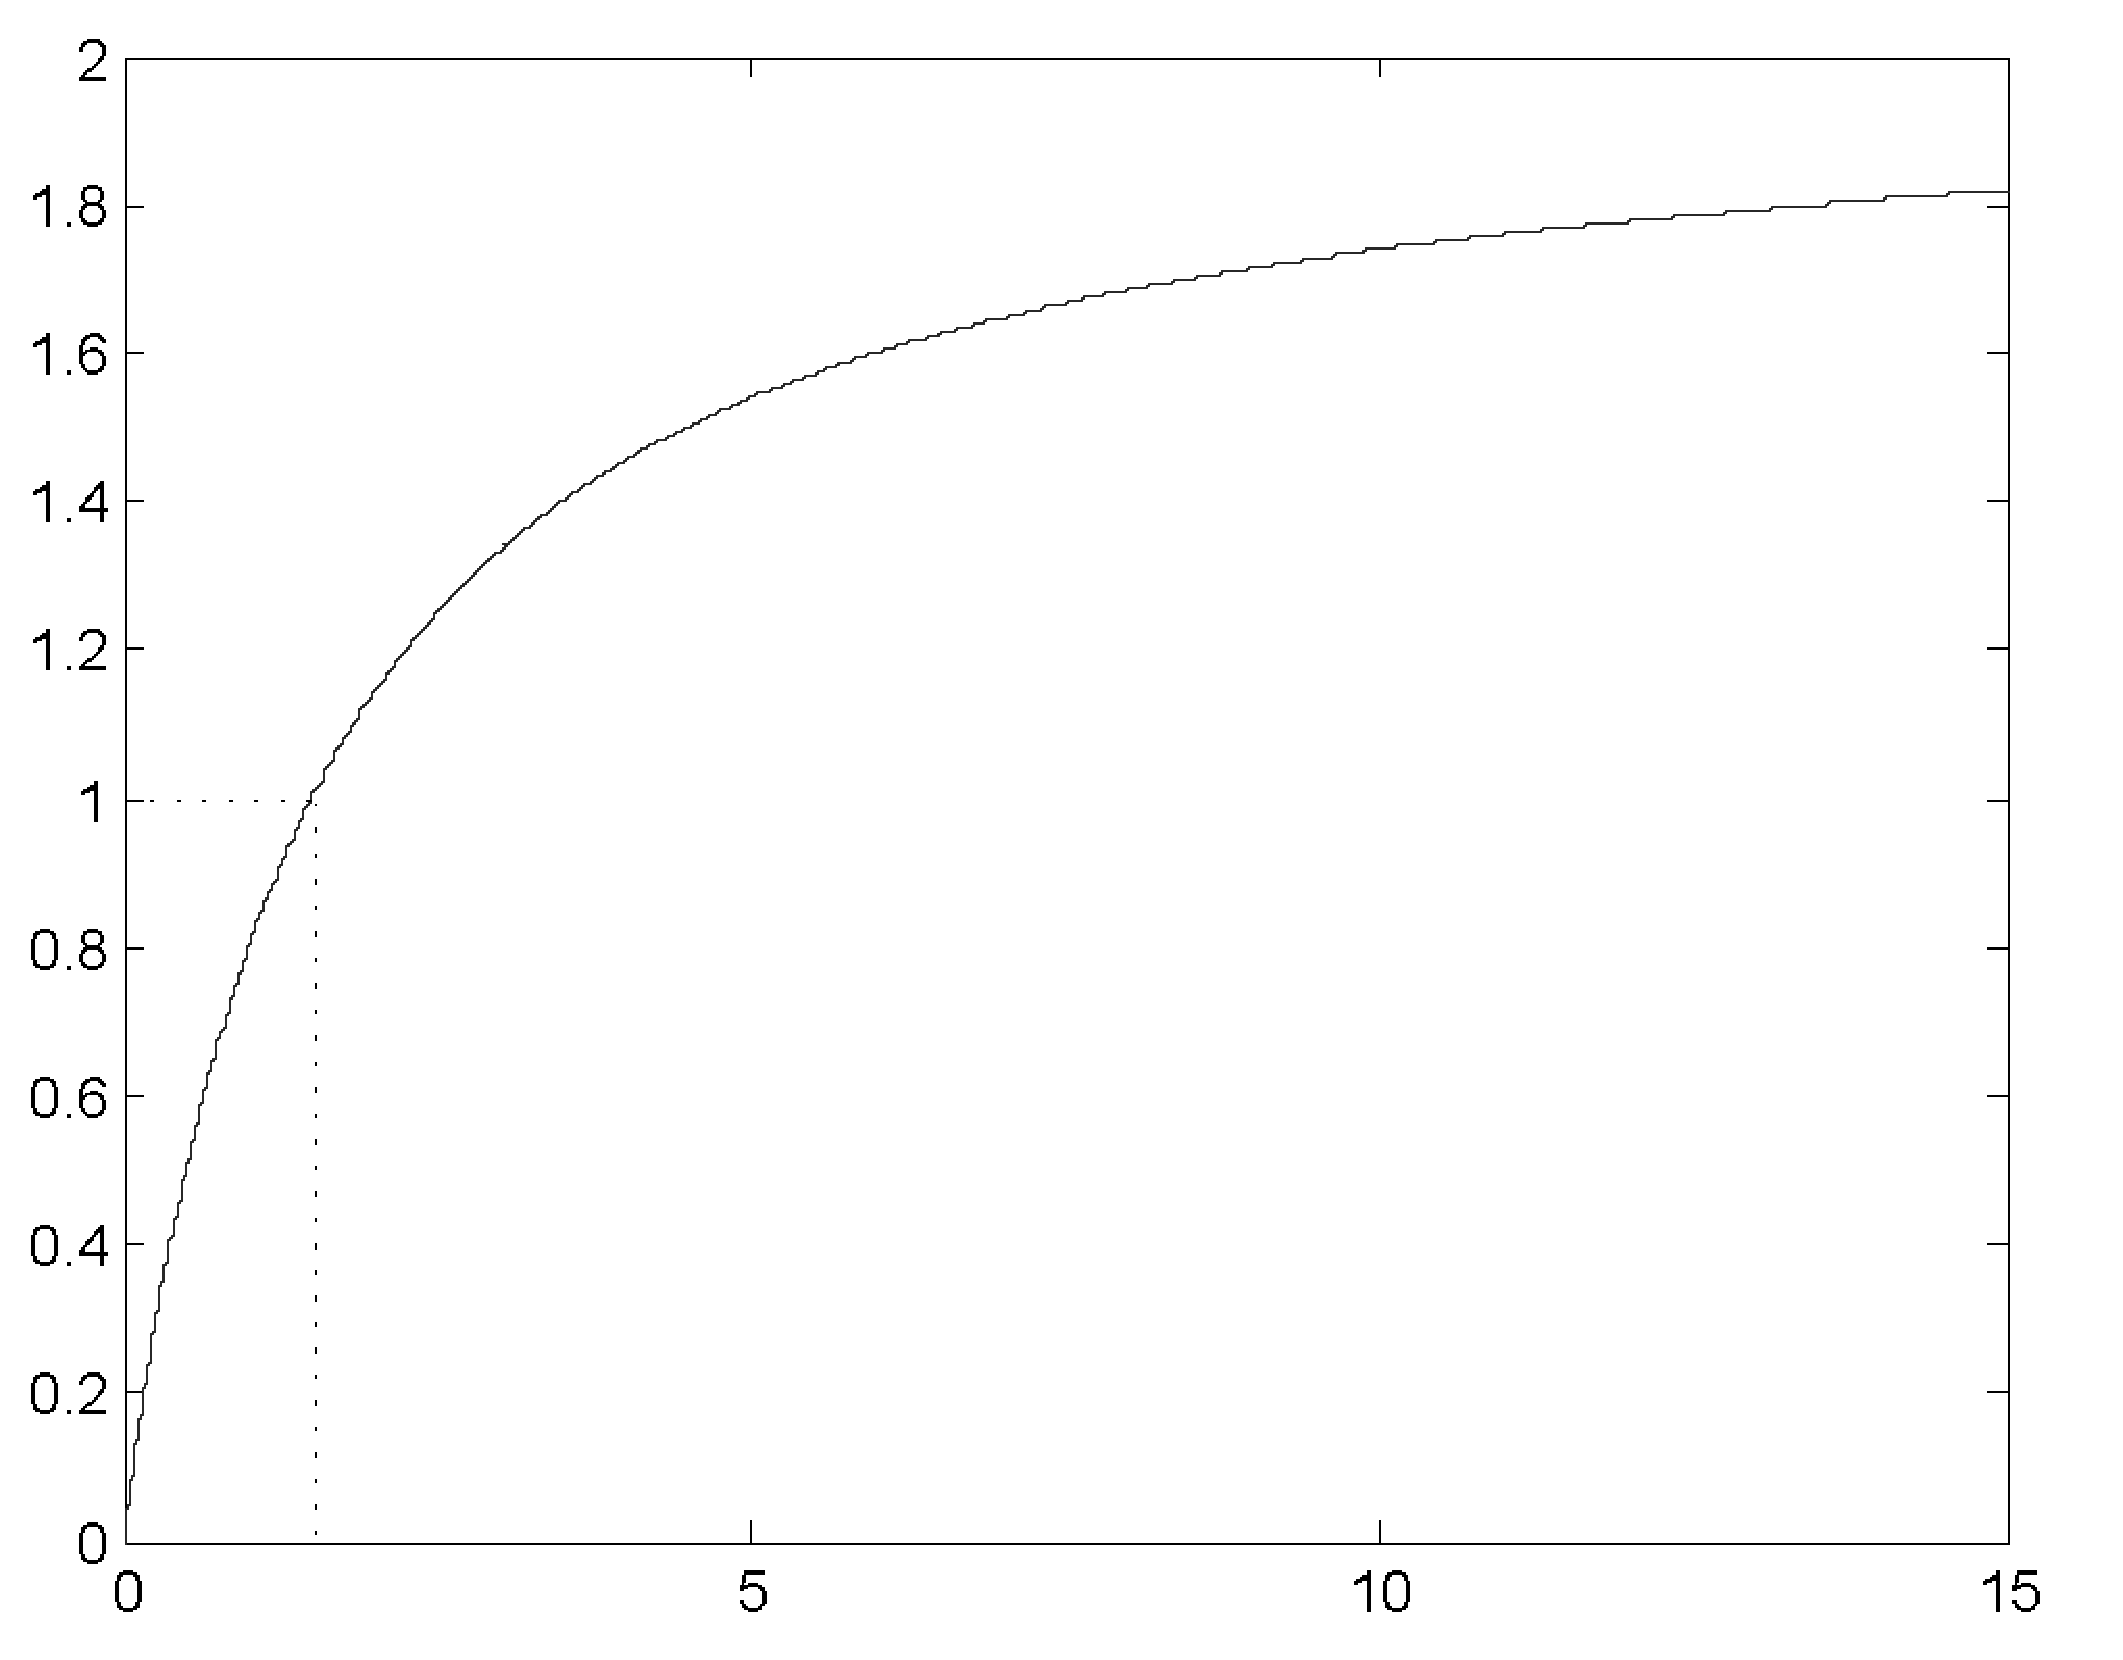
\includegraphics[width=0.5\textwidth]{../figs_05_chemostat/monod}
\caption{A typical Monod growth curve.}
\end{center}
\label{fig:monod_curve}
\end{figure}
From now on, we assume a Monod function. 
In other contexts, this curve is called a Holling Type II function.


\subsection{Equilibria}
To compute the equilibria, suppose $S'=x'=0$, giving
\[
\mu(S)x=-\mu(S)x=0.
\]
This implies $\mu(S)=0$ or $x=0$. Note that $\mu(S)=0\Leftrightarrow S=0$, so the system is at equilibrium if $S=0$ or $x=0$.

This is a complicated situation, as it implies that there are lines of
equilibria ($S=0$ and any $x$, and $x=0$ and any $S$), so that the equilibria
are not \emph{isolated} (arbitrarily small neighborhoods of one equilibrium
contain other equilibria), and therefore, studying the linearization is not
possible.
Here, some analysis is however possible.
Consider
\[
\frac{dx}{dS}=\frac{dx}{dt}\frac{dt}{dS}=-\frac{\mu(S)x}{\mu(S)x}=-1.
\]
This implies that we can find the solution
\[
x(S)=C-S,
\]
or, supposing the initial condition is $(S(0),x(0))=(S_0,x_0)$, that is, $x(S_0)=x_0$,
\begin{equation}\label{eq:sol_chemostat_batch_no_death}
x(S)=S_0+x_0-S.
\end{equation}
\begin{figure}[htbp]
\begin{center}
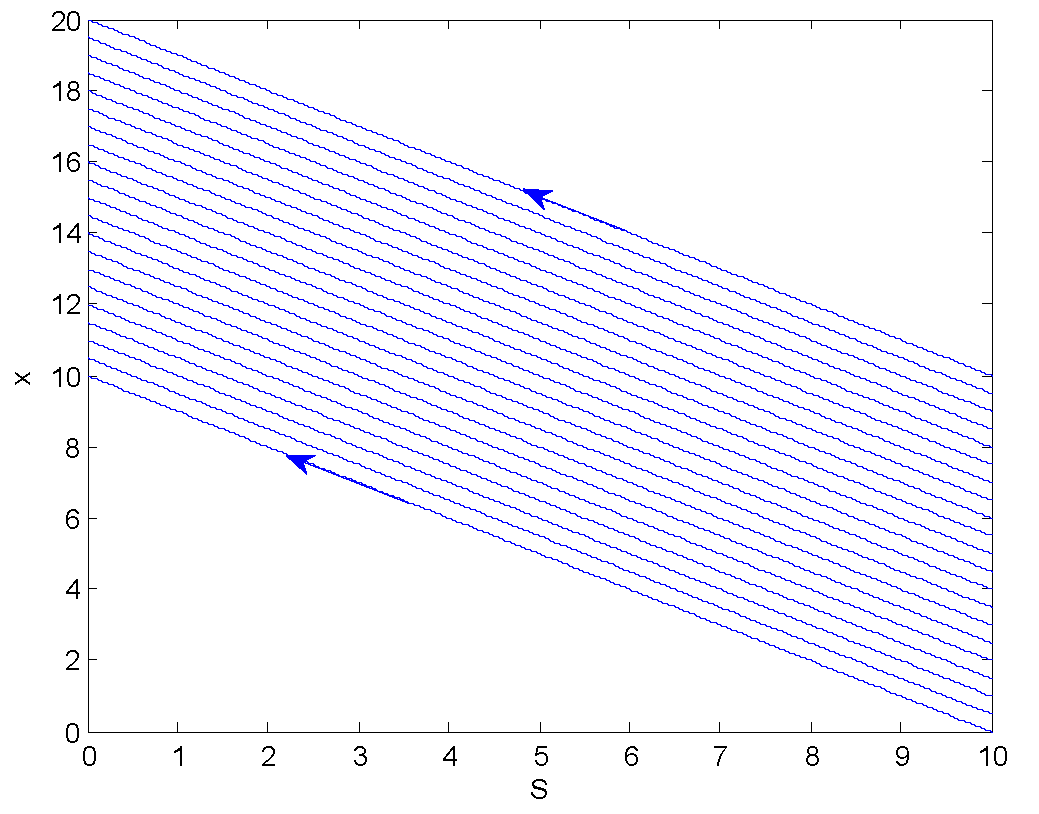
\includegraphics[width=0.5\textwidth]
{../figs_05_chemostat/chemo_batch_nodeath_Sx}
\caption{Typical solutions obtained from
\eqref{eq:sol_chemostat_batch_no_death}.}
\end{center}
\end{figure}




\subsection{Model with organism death}
Assume death of organisms at per capita rate $d$. Model is
\begin{subequations}\label{sys:chemo_batch_death}
\begin{align}
S' &= -\mu(S)x \\
x' &= \mu(S)x-dx.
\end{align}
\end{subequations}
We have
\[
S'=0\Leftrightarrow \mu(S)x=0
\]
and
\[
x'=0\Leftrightarrow (\mu(S)-d)x=0.
\]
So we have $x=0$ or $\mu(S)=d$. So $x=0$ and any value of $S$, and $S$ such that $\mu(S)=d$ and $x=0$. One such particular value is $(S,x)=(0,0)$.
This is once again a complicated situation, since there are lines of equilibria. Intuitively, most solutions will go to $(0,0)$. This is indeed the case (we will not show it).



\section{Continous flow mode}
\subsection{Modelling principles}
General hypotheses are similar to the batch case, except that additionally,
\begin{itemize}
\item Limiting substrate (whose concentration in the vessel is denoted $S$) is input at the rate $D$ and concentration $S^0$.
\item There is an outflow of both nutrient and organisms (at same rate $D$ as input). 
\item Residence time in device is assumed small compared to lifetime (or time to division) $\Rightarrow$ no death considered.
\end{itemize}

\begin{figure}[htbp]
\begin{center}
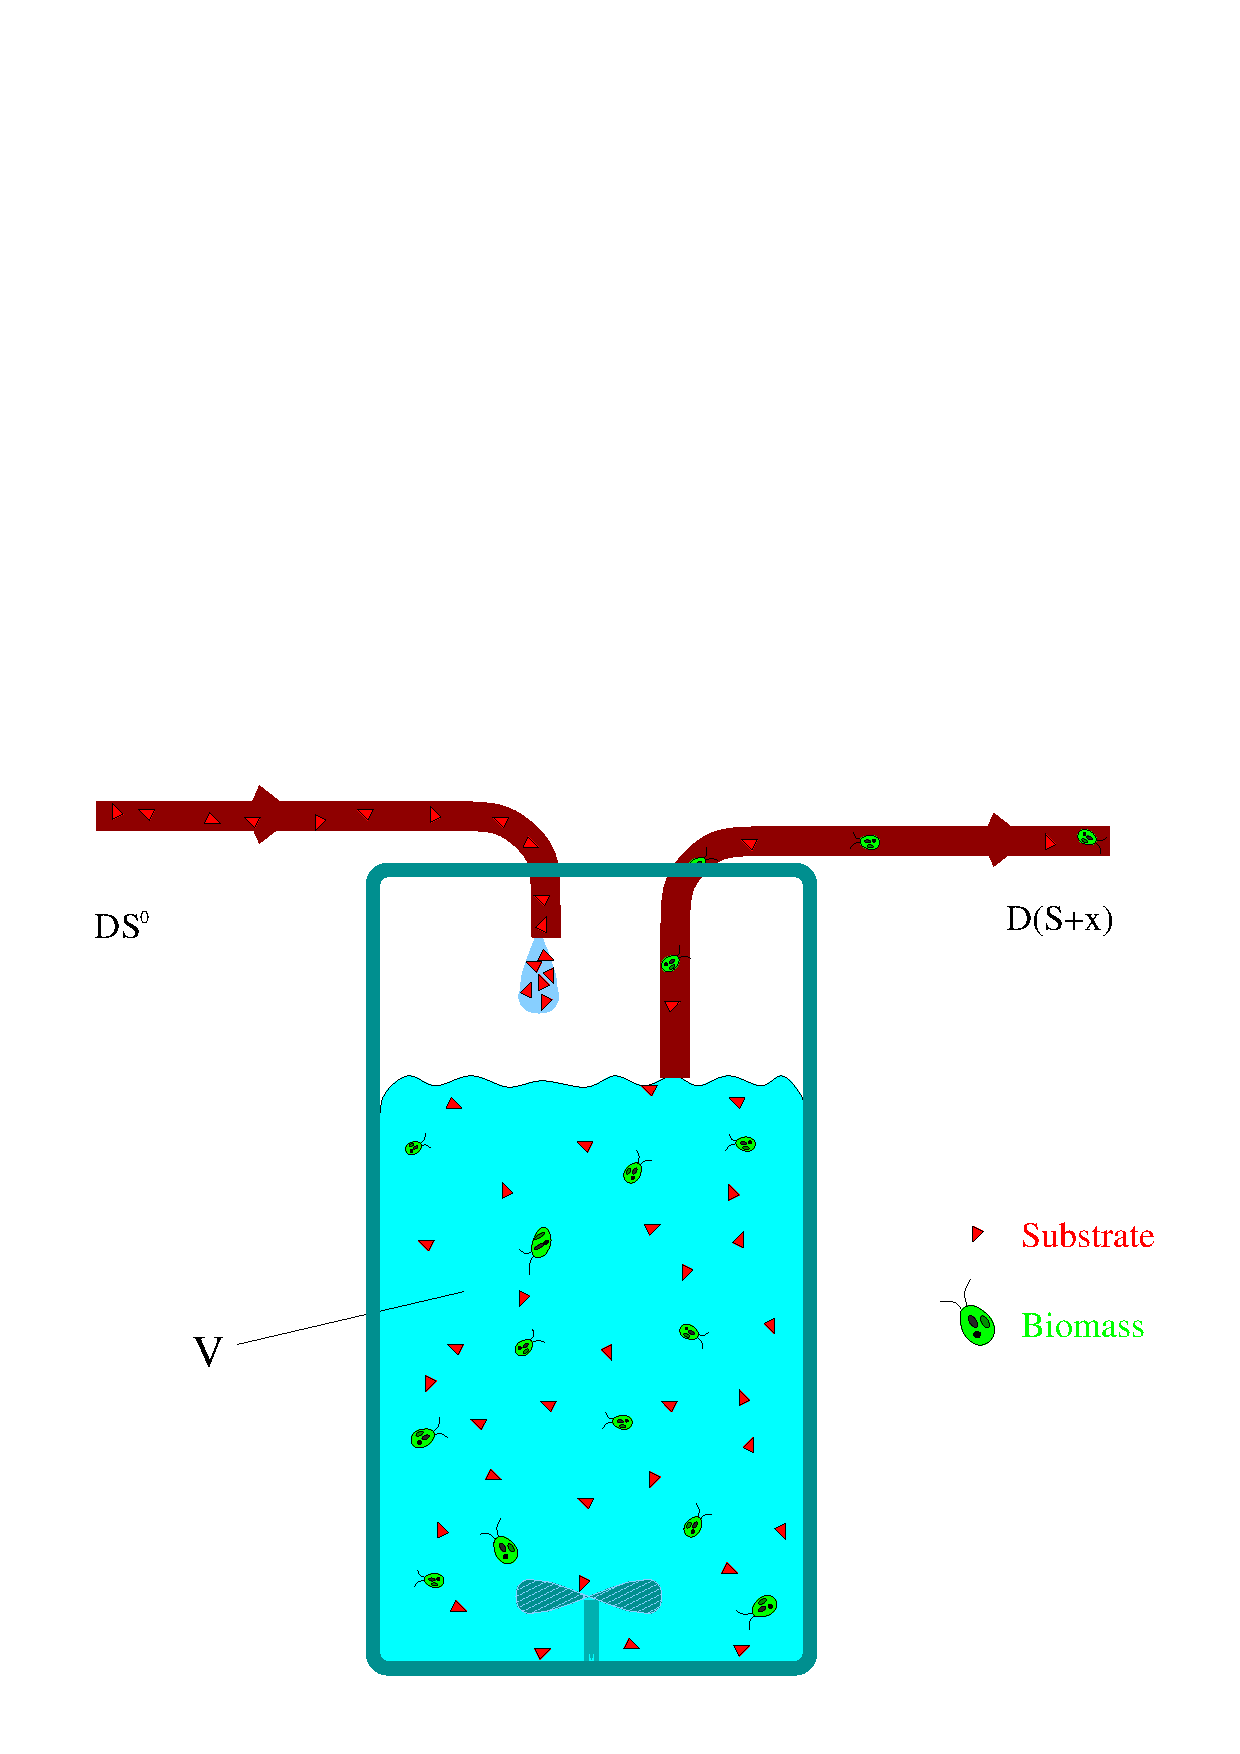
\includegraphics[height=0.45\textwidth]{../figs_05_chemostat/figchemo_eng}
\caption{A schematic representation of a chemostat operating in continuous flow
mode.}
\label{fig:schema_chemostat_CSTR}
\end{center}
\end{figure}


\subsection{Model for continuous flow mode}
The model is
\begin{subequations}\label{sys:chemo_flow}
\begin{align}
S' &= D(S^0-S)-\mu(S)x \\
x' &= \mu(S)x-Dx,
\end{align}
\end{subequations}
with initial conditions $S(0)\geq 0$ and $x(0)\geq 0$, and $D,S^0>0$. This is called the \emph{Monod model}.


\subsection{Finding equilibria}
Setting $S'=x'=0$, we get
\begin{align*}
0&=D(S^0-S)-\mu_{max}\frac{S}{K_S+S}x \\
0&=\left(\mu_{max}\frac{S}{K_S+S}-D\right)x
\end{align*}
But here, instead of directly computing the values of the equilibrium points, we consider the system in the plane, using nullclines.


\subsection{Phase plane analysis}
Nullclines are the level set 0 of the vector field. If we have
\begin{align*}
x_1' &= f_1(x_1,x_2) \\
x_2' &= f_2(x_1,x_2)
\end{align*}
then the nullclines for $x_1$ are the curves defined by 
\[
\{(x_1,x_2)\in\IR^2:f_1(x_1,x_2)=0\},
\]
those for $x_2$ are
\[
\{(x_1,x_2)\in\IR^2:f_2(x_1,x_2)=0\}.
\]
(Note: In $\IR^2$, nullclines are curves.)
On the nullcline associated to one state variable, this state variable has zero derivative.
Equilibria lie at the intersections of nullclines for both state variables (in $\IR^2$).

\frame{\frametitle{Nullclines for $x$}
Nullclines are given by
\begin{subequations}
\begin{align}
0&=D(S^0-S)-\mu_{max}\frac{S}{K_S+S}x \label{eq:ncS}\\
0&=\left(\mu_{max}\frac{S}{K_S+S}-D\right)x \label{eq:ncx}
\end{align}
\end{subequations}
From \eqref{eq:ncx}, nullclines for $x$ are $x=0$ and 
\[
\mu_{max}\frac{S}{K_S+S}-D=0
\]
Write the latter as
\begin{align*}
\mu_{max}\frac{S}{K_S+S}-D=0 &\Leftrightarrow \mu_{max}S=D(K_S+S) \\
&\Leftrightarrow (\mu_{max}-D)S=DK_S \\
&\Leftrightarrow S=\frac{DK_S}{\mu_{max}-D}
\end{align*}
}

\frame{\frametitle{Nullcline for $x$}
So, for $x$, there are two nullclines:
\begin{itemize}
\item The line $x=0$.
\item The line $S=\dfrac{DK_S}{\mu_{max}-D}$.
\end{itemize}
For the line $S=DK_S/(\mu_{max}-D)$, we deduce a condition:
\begin{itemize}
\item If $\mu_{max}-D>0$, that is, if $\mu_{max}>D$, i.e., the maximal growth rate of the cells is larger than the rate at which they leave the chemostat due to washout, then the nullcline intersects the first quadrant.
\item If $\mu_{max}<D$, then the nullcline does not intersect the first quadrant. 
\end{itemize}
}

\frame{\frametitle{Nullclines for $S$}
Nullclines are given by
\begin{subequations}
\begin{align}
0&=D(S^0-S)-\mu_{max}\frac{S}{K_S+S}x \tag{\ref{eq:ncS}}\\
0&=\left(\mu_{max}\frac{S}{K_S+S}-D\right)x \tag{\ref{eq:ncx}}
\end{align}
\end{subequations}
Rewrite \eqref{eq:ncS},
\begin{align*}
D(S^0-S)-\mu_{max}\frac{S}{K_S+S}x=0 &\Leftrightarrow 
\mu_{max}Sx=D(S^0-S)(K_S+S) \\
&\Leftrightarrow 
x = \frac{D(S^0-S)(K_S+S)}{\mu_{max}S}
\end{align*}
}


\frame{\frametitle{Nullcline for $S$: $S$ intercept}
The equation for the nullcline for $S$ is
\[
x =\Gamma(S)\stackrel{\Delta}{=} \frac{D}{\mu_{max}}\left(\frac{S^0K}S-S+S^0-K\right)
\]
We look for the intercepts. First, $S$ intercept:
\begin{align*}
\Gamma(S)=0 &\Leftrightarrow \frac{S^0K_S}S-S+S^0-K_S=0 \\
&\Leftrightarrow \frac{S^0K}S=S-S^0+K \\
&\Leftrightarrow S^0K_S=S^2+(K_S-S^0)S \\
&\Leftrightarrow S^2+(K-S^0)S-S^0K_S =0
\end{align*}
Roots of this degree 2 polynomial are $-K_S$ ($<0$) and $S^0$.
}

\paragraph{Nullcline for $S$: $x$ intercept}
$x$ intercept is found at $\Gamma(0)$. But this is not defined (division by $S=0$), so consider
\begin{align*}
\lim_{S\to 0^+}\Gamma(S) &= \lim_{S\to 0^+}\frac{D}{\mu_{max}}\left(\frac{S^0K}S-S+S^0-K\right) \\
&= \frac{D}{\mu_{max}}\left(\lim_{S\to 0^+}\frac{S^0K}S-S+S^0-K\right) \\
&= \frac{D}{\mu_{max}}\left(\lim_{S\to 0^+}\left(\frac{S^0K}S\right)+\lim_{S\to 0^+}\left(-S+S^0-K\right)\right) \\
&= \frac{D}{\mu_{max}}\left(+\infty+S^0-K\right) \\
&= +\infty.
\end{align*}


Maple has a plot function, {\tt implicitplot} (part of the {\tt plots} library), that is very useful for nullclines ($d$ is used instead of $D$, because maple does not allow to change $D$ without using {\tt unprotect}).
\begin{verbatim}
> with(plots):
> d := 0.4; S0 := 1; mu := 0.7; K := 2;
> implicitplot(d*(S0-S)-mu*S/(K+S)*x=0,S=0..10,x=0..10)
\end{verbatim}



\subsection{Stability of the equilibria}
The computation was done during class.


\subsection{Conservation of mass}
Summing the equations in \eqref{sys:chemo_flow}, we get
\[
(S+x)'=D\left(S^0-(S+x)\right)
\]
Denote $M=S+x$ the total organic mass in the chemostat. Then
\[
M'=D(S^0-M)
\]
This is a linear equation in $M$. Solving it (e.g., integrating factor), we find
\[
M(t)=S^0-e^{-Dt}\left(S^0-M(0)\right),
\]
and so
\[
\lim_{t\to\infty}M(t)=S^0.
\]
This is called the \emph{mass conservation principle}.

\paragraph{Implication of mass conservation}
Not as strong as what we had in the SIS epidemic model, where the total number of individuals was constant. Here, the mass is \emph{asymptotically} constant.
{\bf But} we can still use it, using the theory of \emph{asymptotically autonomous} differential equations. Too complicated for here, just remember that often, it is \emph{allowed} to use the limit of a variable rather than the variable itself, provided you know that the convergence occurs.

